\chapter{Narzędzia}
\section{Formaty zapisu grafów} \label{sec:graph-formats}
Istnieje wiele formatów służących do reprezentowania grafów. W ciągu ostatnich dwóch dekad zostało zaproponowanych lub było używanych prawie 100 różnych formatów \cite{roughan-tuke}. Różnią się one przede wszystkim strukturą (XML, JSON) oraz możliwościami (np. wsparcie dla grafów hierarchicznych czy hipergrafów).

Do najpopularniejszych formatów należą \cite{bernard,gephi}:

\begin{itemize}
\setlength\itemsep{0em}
\item GML -- \textit{Graph Modeling Language }
\item XGMML -- \textit{eXtensible Graph Markup and Modeling Language}
\item GraphML -- \textit{Graph Markup Language}
\item GEXF -- \textit{Graph Exchange XML Format}
\item JGF -- \textit{JSON Graph Format}
\item DOT -- format programu Graphviz
\item DGML -- \textit{Directed Graph Markup Language}
\end{itemize}

\subsubsection{Graph Markup Language (GraphML)}

GraphML jest formatem zapisu grafów bazującym na składni XML. Format ten wspiera wszystkie typy grafów (skierowane, nieskierowane, mieszane). Wspiera również hipergrafy oraz grafy hierarchiczne. Dodatkowo umożliwia przypisywanie do wierzchołków i krawędzi atrybutów zawierających dane specyficzne dla aplikacji.

GraphML jest następcą formatu GML (nie będącego standardem XML). Prace nad formatem GML zostały zapoczątkowane przez społeczność \textit{Graph Drawing} podczas Sympozjum Rysowania Grafów w 1995 roku w Pasawie w Niemczech. Pięć lat później przed 8. Międzynarodowym Sympozjum Rysowania Grafów w 2000 roku w Williamsburgu w USA ruszyły prace nad nowym formatem GraphML \cite{graphml}.

Plik w formacie GraphML zawiera element \texttt{graph} (graf), który może zawierać elementy \texttt{node} (wierzchołek), \texttt{edge} (krawędź) oraz \texttt{hyperedge} (hiperkrawędź). Każdy element \texttt{node} powinien zawierać unikalny atrybut \texttt{id} (identyfikator), który jest używany do definiowania krawędzi. Każda krawędź posiada atrybuty \texttt{source} (źródło) oraz \texttt{target} (cel), które odpowiadają identyfikatorom wierzchołków i oznaczają odpowiednio początek i koniec krawędzi. Najwyższym elementem w hierarchii jest \texttt{graphml}, który może zawierać serię elementów \texttt{key} (klucz) służących do definiowania atrybutów danych oraz serię elementów \texttt{graph}.

Z formatem tym związane są dwa rozszerzenia: \textit{attribute extension} i \textit{parseinfo extension}. Pierwsze z nich pozwala na wyspecyfikowanie typu atrybutu oraz jego nazwy. Drugie dodaje kilka atrybutów do elementów \texttt{graph} i \texttt{node}, takich jak ilość wierzchołków, ilość krawędzi, maksymalny stopień wierzchołka w grafie czy ilość krawędzi wychodzących dla wierzchołka. Metadane te mają na celu pomóc analizatorom składni (parserom) efektywniej przetwarzać pliki z grafami zapisanymi w formacie GraphML. 

Format GraphML wspierają programy yEd Graph Editor oraz w ograniczonym stopniu Gephi (bez hipergrafów i grafów hierarchicznych).

\vspace*{\fill}
\begin{figure}[h]
\centering
\begin{tikzpicture}
\filldraw 
(0,0) node[label=1](1){}
(2,2) node[label=2](2){} 
(4,0) node[label=3](3){};
\path[draw] (1)--(2);
\path[draw] (2)--(3);
\path[draw] (3)--(1);
\end{tikzpicture}
\caption{} \label{fig:example-graph}
\end{figure}
\vspace*{\fill}

\pagebreak

\begin{listing}[H]
    \caption{Reprezentacja grafu z rysunku \ref{fig:example-graph} w formacie GraphML}
    \inputminted{xml}{example.graphml}
    \label{lst:graphml-example}
\end{listing}

\subsubsection{Graph Exchange XML Format (GEXF)}

GEXF jest formatem opierającym się na XML, który służy do opisywania struktur złożonych sieci, związanych z nimi danych oraz zmian zachodzących w czasie. Został stworzony w 2007 roku na potrzeby aplikacji Gephi.  

Format GEXF wspiera wszystkie typy grafów (skierowane, nieskierowane, mieszane). Wspiera też grafy hierarchiczne, ale nie wspiera hipergrafów. W GEXF jest możliwe przypisywanie do wierzchołków i krawędzi dowolnych atrybutów. 

W formacie tym najwyższym elementem w hierarchii jest element \texttt{graphml}. Zawiera on jeden element \texttt{graph}, który zawiera elementy \texttt{attributes}, \texttt{nodes} i \texttt{edges}, służące kolejno do definiowania atrybutów, wierzchołków i krawędzi. Element \texttt{node} (znajdujący się w \texttt{nodes}) podobnie jak w formacie GraphML posiada unikalny atrybut \texttt{id}, a element \texttt{edge} (znajdujący się w \texttt{edges}) posiada atrybuty \texttt{source} oraz \texttt{target} odpowiadające wartościom atrybutów \texttt{id} elementów \texttt{node} i oznaczające odpowiednio początek i koniec krawędzi.  

\begin{listing}[H]
    \caption{Reprezentacja grafu z rysunku \ref{fig:example-graph} w formacie GEXF}
    \inputminted{xml}{example.gexf}
    \label{lst:gexf-example}
\end{listing}

\subsubsection{JSON Graph Format (JGF)} 

JSON Graph Format jest specyfikacją służącą do reprezentowania grafów, która korzysta z formatu JSON (ang. \textit{JavaScript Object Notation}). Specyfikacja ta powstała w 2014 roku. 

Korzystając z JGF możemy przedstawiać grafy skierowane lub nieskierowane. Format ten nie wspiera grafów hierarchicznych ani hipergrafów. Podobnie jak w dwóch powyższych formatach do wierzchołków oraz krawędzi możemy przypisywać dowolne atrybuty. 

W obiekcie JSON będącym w formacie JGF główną właściwością jest \texttt{graph} lub \texttt{graphs}, których wartościami są odpowiednio obiekt lub tablica obiektów reprezentujących graf. Obiekt ten (lub obiekty) posiadają właściwości \texttt{nodes} oraz \texttt{edges}. Ich wartościami są tablice zawierające obiekty opisujące odpowiednio wierzchołki oraz krawędzie grafu. Podobnie jak w dwóch poprzednich formatach wierzchołki mają właściwość \texttt{id}, a krawędzie \texttt{source} oraz \texttt{target} oznaczające początek i koniec krawędzi. 

\begin{listing}[H]
    \caption{Reprezentacja grafu z rysunku \ref{fig:example-graph} w formacie JGF}
    \inputminted{json}{example.json}
    \label{lst:jgf-example}
\end{listing}

\subsubsection{DOT Graphviz} 

DOT jest formatem tekstowym służącym do opisu grafu. Powstał w roku 2000. Wspiera wszystkie typy grafów (skierowane, nieskierowane, mieszane). W formacie tym możliwe jest również reprezentowanie grafów hierarchicznych, ale nie jest możliwe przedstawianie hipergrafów. W DOT możemy przypisywać do wierzchołków i krawędzi dowolne atrybuty.  

Format ten jest formatem czytelnym dla człowieka. Zdefiniowana jest gramatyka bezkontekstowa opisująca ten format, która może być zapisana przy pomocy notacji BNF (ang. \textit{Backus-Naur Form}).

Definicja grafu rozpoczyna się od słowa kluczowego \texttt{graph} lub \texttt{digraph}. Po nim następują nawiasy klamrowe, wewnątrz których znajduje się opis wierzchołków i krawędzi. Podwójna pauza (\texttt{-{}-}) oznacza krawędź nieskierowaną, a strzałka (\texttt{->}) oznacza krawędź skierowaną.

Format ten jest obsługiwany przez program Graphviz.

\bigskip

\begin{listing}[H]
    \caption{Reprezentacja grafu z rysunku \ref{fig:example-graph} w formacie DOT}
    \inputminted{text}{example.gv}
    \label{lst:dot-example}
\end{listing}

\begin{table}[H]
\caption{Porównanie formatów GraphML, GEXF, JGF oraz DOT}
\label{tab:formats-comparison}
\begin{tabularx}{\textwidth}{ r|Y|Y|Y|Y| } 
\multicolumn{1}{r}{}
 & \multicolumn{1}{c}{\rotatebox{45}{GraphML}}
 & \multicolumn{1}{c}{\rotatebox{45}{GEXF}} 
 & \multicolumn{1}{c}{\rotatebox{45}{JGF}} 
 & \multicolumn{1}{c}{\rotatebox{45}{DOT}} 
\\\cline{2-5}

struktura
 & {\footnotesize XML}
 & {\footnotesize XML} 
 & {\footnotesize JSON}  
 & {\footnotesize BNF}
\\\cline{2-5}

grafy skierowane 
 & \checkmark
 & \checkmark  
 & \checkmark  
 & \checkmark 
\\\cline{2-5}

grafy nieskierowane  
 & \checkmark 
 & \checkmark  
 & \checkmark  
 & \checkmark  
\\\cline{2-5}

grafy mieszane  
 & \checkmark 
 & \checkmark  
 & --  
 & \checkmark  
\\\cline{2-5}

multigrafy 
 & \checkmark 
 & \checkmark  
 & \checkmark  
 & \checkmark  
\\\cline{2-5}

grafy hierarchiczne 
 & \checkmark 
 & \checkmark  
 & --  
 & \checkmark
\\\cline{2-5}

hipergrafy 
 & \checkmark 
 & --  
 & --  
 & -- 
\\\cline{2-5}

dowolne atrybuty 
 & \checkmark 
 & \checkmark  
 & \checkmark  
 & \checkmark 
\\\cline{2-5}

wartości domyślne atrybutów 
 & \checkmark 
 & \checkmark  
 & --  
 & \checkmark  
\\\cline{2-5}

wiele grafów 
 & \checkmark 
 & --  
 & \checkmark  
 & -- 
\\\cline{2-5}

zmiana grafu w czasie 
 & -- 
 & \checkmark  
 & --  
 & --  
\\\cline{2-5}
\end{tabularx}
\end{table}

\pagebreak

\section{Biblioteki do wizualizacji grafów w JavaScript}

W tej sekcji opiszę i porównam najbardziej znane biblioteki w JavaScript służące do wyświetlania grafów: Cytoscape.js, Sigma (oraz jej rozszerzenie Linkurious.js) i VivaGraphJS. 

Istnieje wiele bibliotek, które służą do wizualizacji danych w ogólności (np. wykresów liniowych, kołowych, słupkowych, osi czasu, schematów). Dobrymi przykładami są tutaj dwie popularne biblioteki: D3.js oraz vis.js. Jednakże skupię się jedynie na tych bibliotekach, które służą tylko i wyłącznie do wizualizacji grafów. Po pierwsze dlatego, że oferują one większe możliwości do analizowania i przetwarzania grafów. Po drugie, są lepiej przystosowane do obsługi dużych grafów pod względem wydajności. 

Innymi ciekawymi bibliotekami są Graphosaurus oraz ngraph.pixel. Służą one do wyświetlania grafów w trzech wymiarach. Jednakże ich opis również pozwolę sobie pominąć, ponieważ tematyka ta wchodzi poza zakres tej pracy.

\subsection{Cytoscape.js}

Cytoscape.js jest biblioteką z otwartym źródłem (ang. \textit{open-source}) do analizy i wizualizacji grafów. Udostępniona na zasadach licencji MIT. Została napisana w czystym JavaScript i nie posiada zależności do żadnych innych bibliotek. Cytoscape.js jest następcą porzuconego projektu Cytoscape Web korzystającego z technologii Adobe Flash \cite[309]{franz}. 

Prawa własności intelektualnej posiada do niej Cytoscape Consortium -- organizacja \textit{non profit}, która promuje rozwój i dystrybucję oprogramowania związanego z sieciami biologicznymi. Cytoscape.js została stworzona na University of Toronto. Jej głównym kontrybutorem jest Max Franz. Biblioteka została sfinansowana przez granty NRNB (\textit{National Resource for Network Biology}) i NIH (\textit{National Institutes of Health}). Kilka innych uniwersytetów oraz firm również pomagało w rozwoju biblioteki \cite{cytoscape}. 

Cytoscape.js jest kompatybilny z najpopularniejszymi bibliotekami oraz środowiskami JavaScript, takimi jak: Node.js, Browserify, webpack, RequireJS czy Bower. Pozwala to na integrację z wieloma systemami napisanymi w JavaScript. 

Architektura Cytoscape.js pozwala na uruchomienie zarówno bez graficznego interfejsu użytkownika oraz jako komponent graficzny, którego implementacja bazuje na elemencie HTML5 Canvas (przykład przedstawiony jest na rysunku \ref{fig:cytoscape}). Umożliwia to korzystanie z biblioteki zarówno po stronie klienta (np. przeglądarka internetowa), jak i po stronie serwera (np. Node.js).

\begin{figure}[H]
\centering
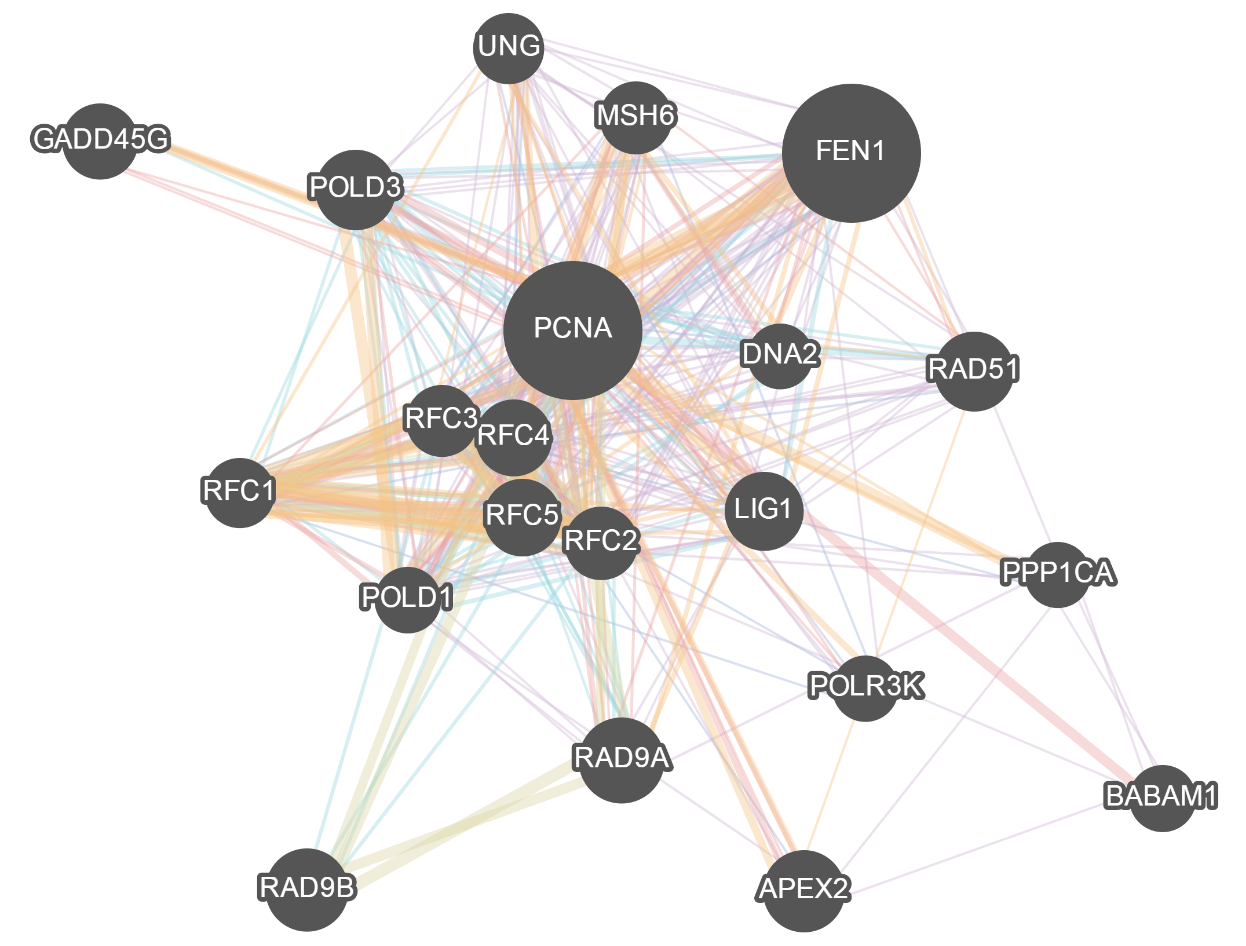
\includegraphics[width=0.7\textwidth]{cytoscape.png}
\captionsetup{justification=centering}
\caption{Przykład wizualizacji grafu w Cytoscape.js -- krawędzie mogą mieć różny kolor i grubość, pomiędzy wierzchołkami może istnieć wiele krawędzi oraz wierzchołki mogą mieć różny rozmiar}\label{fig:cytoscape}
\end{figure}

Cytoscape.js wspiera różne typy grafów: skierowane, nieskierowane, multigrafy. Pozwala na dodawanie, usuwanie i modyfikację krawędzi oraz wierzchołków. Biblioteka dostarcza również możliwość grupowania wierzchołków. W Cytoscape.js istnieje możliwość nadawania wierzchołkom i krawędziom wyglądu poprzez reguły, które są zbliżone do kaskadowych arkuszy styli (CSS, ang. \textit{Cascading Style Sheets}).

W bibliotece jest zaimplementowanych kilka znanych algorytmów takich jak znajdowanie najkrótszej ścieżki, minimalnego drzewa rozpinającego czy minimalnego przekroju. 

Grafy możemy importować i eksportować do formatu JSON. Biblioteka umożliwia również zapis grafu do obrazka (PNG lub JPG). Istnieje też dodatek, który pozwala na zapisywanie i odczytywanie z formatu GraphML. Cytoscape.js jest rozszerzalna -- istnieje możliwość dopisania swoich własnych dodatków (algorytmów, układów, itp).  W chwili obecnej zostało napisanych 30 dodatków zwiększających możliwości biblioteki. 

Cytoscape.js posiada wsparcie dla gestów myszy i gestów na urządzeniach z ekranami dotykowymi. Biblioteka daje możliwość wiązania zdarzeń (ang. \textit{event binding}), np. możemy zdefiniować jaka akcja ma się wykonać po kliknięciu na wierzchołek. 

W Cytoscape.js możemy przesuwać wierzchołki, zmieniać widok przez przeciąganie lub przybliżanie i oddalanie. Istnieje również możliwość zastosowania animacji na całym widoku lub na konkretnych elementach grafu. W~bibliotekę jest wbudowanych kilka automatycznych układów wierzchołków (ang. \textit{layouts}): losowy, siatki (ang. \textit{grid}), okręgu, koncentryczny, zdefiniowany przez przeszukiwanie grafu wszerz (ang. breadth-first search), układ \textit{cose} (\textit{Compound Spring Embedder} -- korzystający z symulacji fizycznej) lub zdefiniowany przez programistę. 

Biblioteka jest w stanie obsłużyć i wyrenderować grafy posiadające tysiące elementów \cite[310]{franz}. Wydajność zależy od urządzenia, na którym jest uruchamiany kod, od silnika JS, rozmiaru grafu oraz użytych styli. W~szczególności kosztowne do wyrenderowania są krawędzie, zwłaszcza w multigrafach ze względu na konieczność narysowania krzywych beziera. W dokumnetacji online jest wiele wskazówek dotyczących optymalizacji pod kątem wydajności (\cite{cytoscape} sekcja \textit{Performance}).

Cytoscape.js posiada obszerną dokumentację online, która zawiera szczegółowy opis API (ang. \textit{Application Programming Interface} -- interfejs programistyczny), przykłady kawałków kodu oraz działające przykłady. 

\subsection{Sigma}

Sigma jest biblioteką dedykowaną do rysowania grafów w aplikacjach internetowych. Powstała w roku 2012. Jej głównymi twórcami są Alexis Jacomy i Guillaume Plique. Udostępniona jest na licencji MIT. 

Sigma dostarcza wiele wbudowanych funkcjonalności takich jak sposób renderowania za pomocą SVG, Canvas lub WebGL czy obsługa gestów myszy i dotyku. Istnieje również możliwość rozszerzenia funkcjonalności przez dopisanie swoich własnych dodatków. 

W repozytorium kodu jest dostępnych 19 oficjalnych dodatków rozszerzających możliwości biblioteki, m.in. parser JSON i GEXF, układy \textit{ForceAtlas2} (bazujący na oddziaływaniu sił pomiędzy wierzchołkami) i \textit{noverlap} (zapewniający, że wierzchołki nie zachodzą na siebie), algorytm A* do znajdowania najkrótszej ścieżki czy algorytm HITS do oceny stron internetowych (podział na autorytety -- strony linkowane i koncentratory -- strony linkujące). 

Innym ciekawym dodatkiem jest dodatek \texttt{sigma.neo4j.cypher}, który pozwala na uruchamianie zapytań w języku Cypher na grafowej bazie danych Neo4j, zinterpretowaniu odpowiedzi i wypełnieniem grafu. Jest on szczególnie warty uwagi ze względu na rosnące znaczenie grafowych baz danych. 

\bigskip

\begin{figure}[H]
\centering
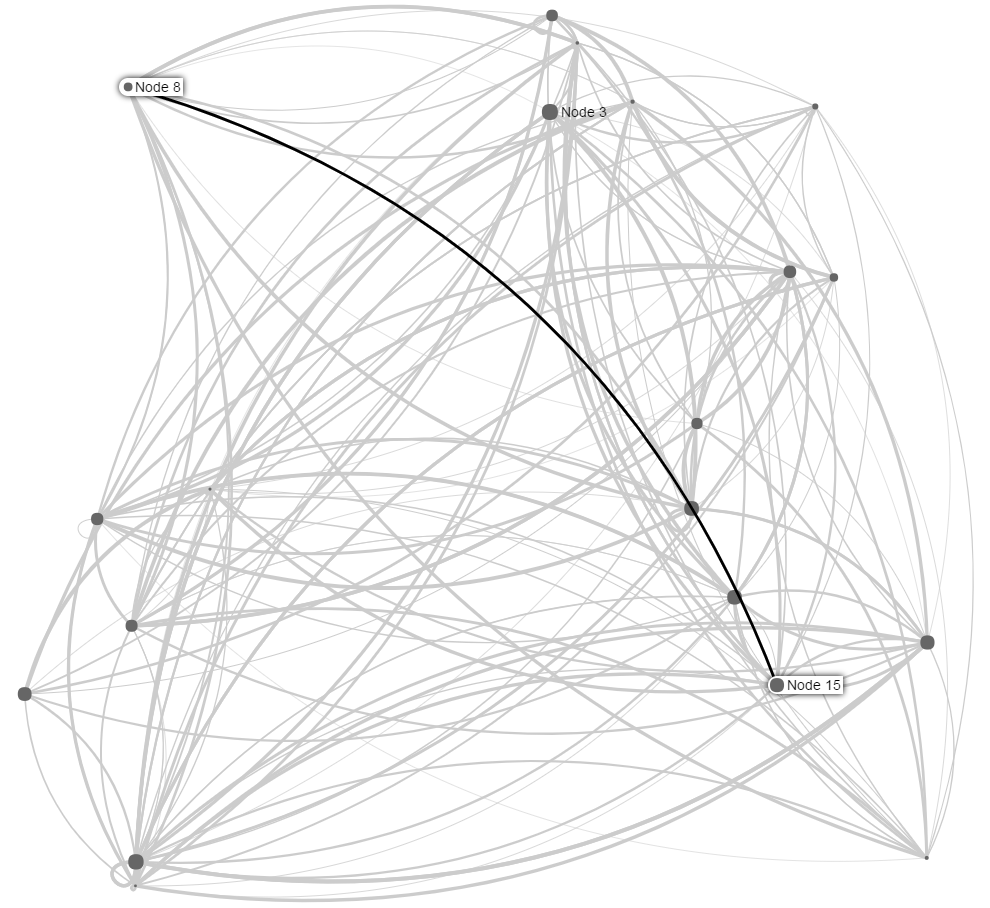
\includegraphics[width=0.7\textwidth]{sigma.png}
\captionsetup{justification=centering}
\caption{Przykładowy graf wyświetlony za pomocą Sigmy}\label{fig:cytoscape}
\end{figure}

\bigskip

Biblioteka można używać z menedżerami pakietów (ang. \textit{package managers}) takimi jak bower czy npm oraz z systemami ładowania modułów (ang. \textit{module loaders}), np. webpack czy RequireJS. Jednakże jest związany z tym pewien problem, mianowicie nie ma łatwej możliwości ładowania osobno dodatków (bez zastosowania obejścia w postaci przypisania do globalnej przestrzeni nazw obiektu \texttt{sigma}, co w nowoczesnym JS nie jest podejściem zalecanym). Na stronie repozytorium sigmy istnieje otwarta propozycja poprawy tego problemu (\cite{sigma-repo} \textit{issue} 730 i 871).


\subsection{Linkurious.js}

Linkurious.js jest rozgałęzieniem (ang. \textit{fork}) projektu Sigma stworzonym przez francuską firmę Linkurious SAS w 2014 roku. Dostępna jest na dwóch licencjach GPLv3 oraz na licencji płatnej dla projektów komercyjnych, które nie spełniają założeń licencji GPLv3. 

Biblioteka rozszerza Sigmę o ponad 20 nowych dodatków. Zostały dodane m.in. dodatki służące do eksportowania (GraphML, CSV, XLSX), nowe układy (algorytm Fruchtermana-Reingolda, \textit{dagre} -- do wyświetlania skierowanych grafów acyklicznych oraz drzew, \textit{ForceLink} -- bazujący na \textit{ForceAtlas2}), dodatek dający możliwość zaznaczania wierzchołków lassem, dodatek pozwalający na wyświetlenie grafu ze współrzędnymi geograficznymi na~mapie (korzystający z biblioteki Leaflet), dodatek do wykrywania społeczności w grafie metodą Louvain oraz kilkanaście innych dodatków \cite{linkurious-diff}. 

Linkurious.js została porzucona w październiku 2016 roku na rzecz nowej biblioteki o nazwie Ogma \cite{ogma}.

\bigskip

\begin{figure}[H]
\centering
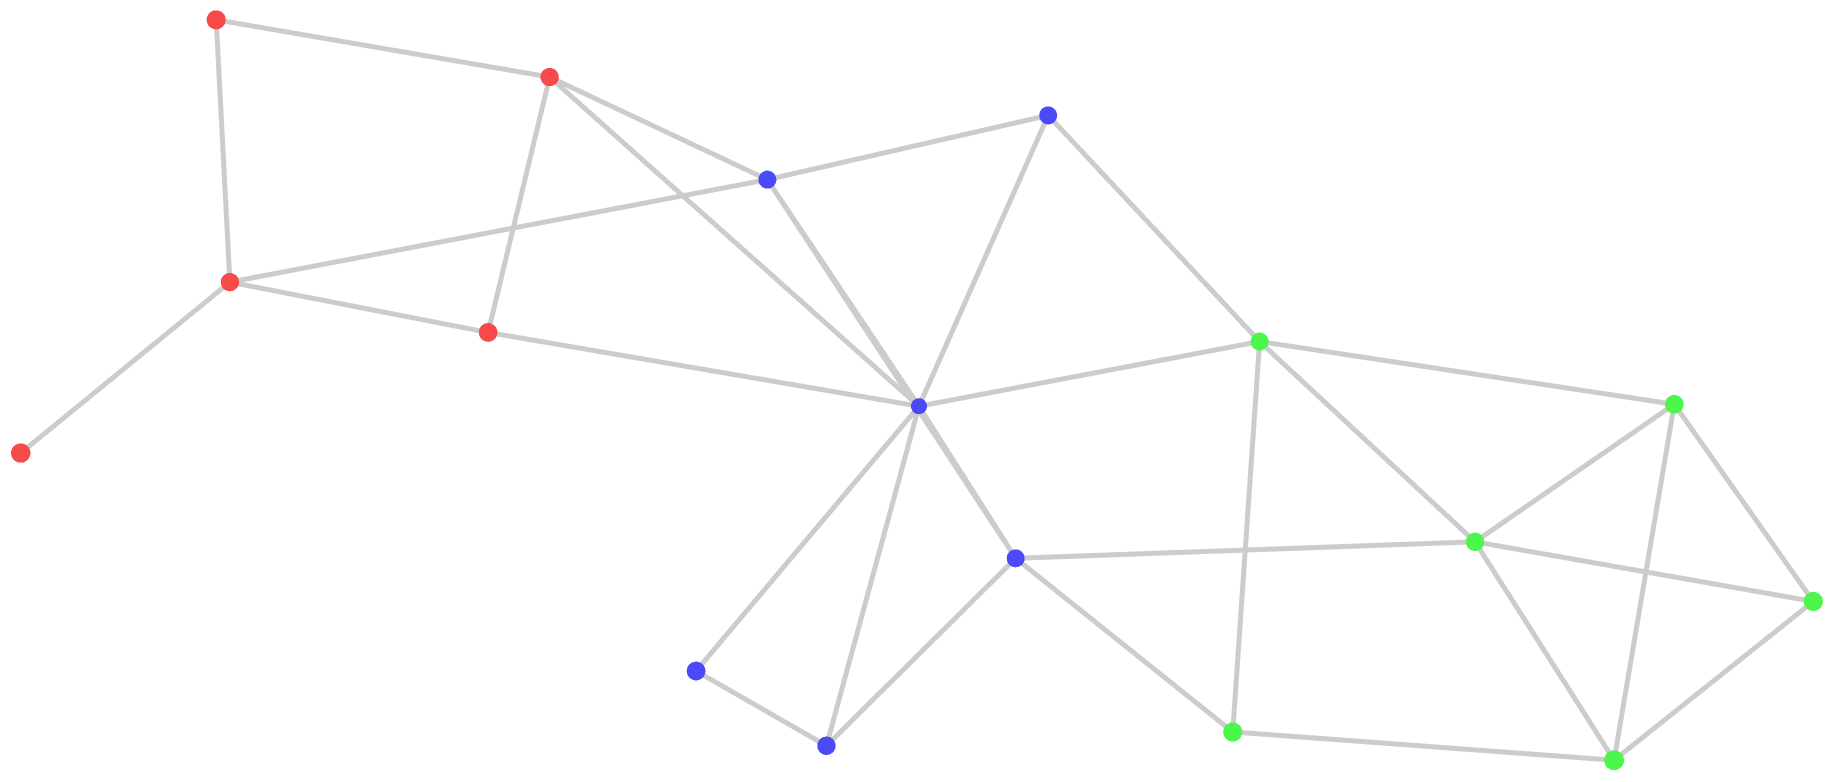
\includegraphics[width=1\textwidth]{linkurious-communities.png}
\captionsetup{justification=centering}
\caption{Przykładowy graf z wykrytymi społecznościami wyświetlony przy pomocy układu \textit{ForceLink} w Linkurious.js}\label{fig:cytoscape}
\end{figure}

\bigskip

\subsection{VivaGraph.js}



\begin{table}[H]
\begin{threeparttable}
\caption{Porównanie bibliotek Cytoscape.js, Sigma, Linkurious.js i VivaGraphJS}
\label{tab:libraries-comparison}
{\renewcommand{\arraystretch}{1.1}
\begin{tabularx}{\textwidth}{ r|Y|Y|Y|Y| } 
\multicolumn{1}{r}{}
 & \multicolumn{1}{c}{\rotatebox{70}{Cytoscape.js}}
 & \multicolumn{1}{c}{\rotatebox{70}{Sigma}} 
 & \multicolumn{1}{c}{\rotatebox{70}{Linkurious.js}} 
 & \multicolumn{1}{c}{\rotatebox{70}{VivaGraphJS}} 
\\\cline{2-5}

rok powstania
 & 2011
 & 2012 
 & 2014
 & 2011 
\\\cline{2-5}

licencja
 & MIT
 & MIT
 & GPLv3\tnote{1} 
 & BSD 3
\\\cline{2-5}

rozszerzalność 
 & \checkmark
 & \checkmark
 & \checkmark   
 & \checkmark  
\\\cline{2-5}

renderowanie SVG 
 & --
 & \checkmark  
 & \checkmark  
 & \checkmark 
\\\cline{2-5}
 
renderowanie Canvas 
 & \checkmark
 & \checkmark  
 & \checkmark  
 & \checkmark  
\\\cline{2-5}

renderowanie WebGL 
 & --
 & \checkmark  
 & \checkmark  
 & \checkmark  
\\\cline{2-5}

obsługa formatu GEXF 
 & --
 & \checkmark  
 & \checkmark  
 & \checkmark
\\\cline{2-5}

obsługa formatu GraphML 
 & \checkmark
 & --
 & \checkmark
 & --
\\\cline{2-5}
\end{tabularx}
}
\begin{tablenotes}
{\footnotesize\medskip
\item[1] lub licencja komercyjna dla projektów nie spełniających założeń licencji GPLv3
}
\end{tablenotes}
\end{threeparttable}
\end{table}


\begin{table}[H]
\caption{Biblioteki Cytoscape.js, Sigma, Linkurious.js i VivaGraphJS -- porównanie statystyk}
\label{tab:libraries-stats-comparison}
{\renewcommand{\arraystretch}{1.1}
\begin{tabularx}{\textwidth}{ r|Y|Y|Y|Y| } 
\multicolumn{1}{r}{}
 & \multicolumn{1}{c}{\rotatebox{70}{Cytoscape.js}}
 & \multicolumn{1}{c}{\rotatebox{70}{Sigma}} 
 & \multicolumn{1}{c}{\rotatebox{70}{Linkurious.js}} 
 & \multicolumn{1}{c}{\rotatebox{70}{VivaGraphJS}} 
\\\cline{2-5}

GitHub -- gwiazdki (ang. \textit{stars}) 
 & 3194
 & 7271
 & 604
 & 2292  
\\\cline{2-5}

GitHub -- kopie projektu (ang. \textit{forks})
 & 466
 & 1150
 & 172  
 & 292  
\\\cline{2-5}

GitHub -- problemy (ang. \textit{issues})
 & 142
 & 376  
 & 28
 & 55  
\\\cline{2-5}

GitHub -- współtwórcy
 & 49
 & 52  
 & 58
 & 14  
\\\cline{2-5}

npm -- instalacje na miesiąc 
 & 12k
 & 1k
 & 281
 & 691  
\\\cline{2-5}

Stack Overflow -- otagowane posty
 & 562
 & 154
 & 23
 & 26  
\\\cline{2-5}
\end{tabularx}
}
\end{table}
